\documentclass{article}

\usepackage[dblblindworkshop]{neurips_2026}
\workshoptitle{World Models in Physical AI}

\usepackage[utf8]{inputenc}
\usepackage[T1]{fontenc}
\usepackage{graphicx}
\usepackage{booktabs}
\usepackage{amsmath}
\usepackage{amsfonts}
\usepackage{microtype}
\usepackage{xcolor}
\usepackage{url}
\usepackage{hyperref}

\title{LateAct: Commitment-Aware Rollback for Asynchronous Control\\
in Interactive Video World Models}

\author{Anonymous Authors}

\newcommand{\method}{\textsc{LateAct}}
\newcommand{\old}{\textsc{Old}}
\newcommand{\new}{\textsc{New}}
\newcommand{\direct}{\textsc{Direct}}
\newcommand{\restart}{\textsc{Restart}}
\newcommand{\nfe}{\textsc{NFE}}

\begin{document}

\maketitle

\begin{abstract}
Interactive video world models are usually evaluated with an action fixed
before generation, yet deployed controllers can change actions while a
few-step diffusion block is already being denoised. We show that this timing
matters: action-conditioned generation can cross an \emph{operational
denoising-time commitment boundary}, after which direct late binding retains
the old action despite using the new action in remaining evaluations. The
observed transition is steep at the few-step sampler's granularity; we do not
assume a universal discrete boundary.
We introduce \method{}, a training-free serving policy that checkpoints the
latest pre-commitment runtime state and recomputes only the necessary denoising
suffix. On Matrix-Game 2.0 mouse-yaw, rollback raises median normalized
new-action response from 0.218 to 0.997. In a frozen asynchronous evaluation on
32 fresh contexts and 1,024 paired arrivals, \method{} matches full restart
within 0.10 response on all 676 late arrivals, uses zero rollback on all 348
early arrivals, and reduces mean late-arrival action-to-pixel latency by
11.93\% with a compact 339,360-byte exact checkpoint. A frozen confirmatory yaw
study on minWM Wan2.1 Action2V passes 16/16 direction-scene gates,
independently replicating the commitment mechanism; we do not test rollback or latency on
minWM. Keyboard controls share the same boundary and recover directional
response, but fail a pre-specified trajectory-fidelity safeguard
(future-SSIM $0.6726<0.90$). Thus \method{} validates commitment-aware rollback
for Matrix-Game mouse-yaw, while cross-model evidence supports the underlying
mechanism rather than universal policy efficacy.
\end{abstract}

\section{Introduction}
\label{sec:intro}

World models promise inexpensive, inspectable rollouts for planning and
control \citep{ha2018worldmodels,hafner2023dreamerv3}. Recent generative
interactive environments can produce action-conditioned pixels
\citep{bruce2024genie,valevski2025gamengen,alonso2024diamond}; few-step causal
video diffusion further moves these systems toward real-time streaming
\citep{he2025matrixgame2,zhao2026minwm}. This progress exposes a serving
question that standard offline evaluations omit: \emph{what happens when a new
action arrives while the current video block is still being denoised?}

A server has three unsatisfactory default choices. It can finish the current
block under the old action, producing stale control feedback; inject the new
action into the remaining denoising evaluations, which is cheap but may be too
late; or restart the block, which recovers control but discards all completed
work. The middle option implicitly assumes that action conditioning remains
equally effective throughout the sampler. Our controlled interventions show
that this assumption is false in two open few-step autoregressive video world
models. The generated branch can become committed to the old action well
before the final denoising evaluation.

This is not the claim that early diffusion steps matter in general. Prior
editing and sampling work already shows that the effect of conditioning can
depend on denoising time. Our question is operational: under identical rollout
state and noise, after how many evaluations does substituting a newly arriving
action cease to recover the new-action outcome? The contribution is the chain
\emph{measurement $\rightarrow$ serving boundary $\rightarrow$ exact suffix
rollback}: we measure action recoverability, turn it into a rollback decision,
and audit the dependencies needed to restore the corresponding runtime state.

We turn this observation into \method{}, a commitment-aware rollback policy.
\method{} measures the latest sampler state from which changing the action
still recovers the new-action oracle, checkpoints exactly that state, and, for
late arrivals, restores it and recomputes only the committed suffix. Early
arrivals bind directly and pay no rollback. The key systems result is that the
necessary Matrix-Game state is not the full live KV allocation: because
current-block cache slices are overwritten before use, an exact checkpoint
contains only the entering-\nfe{}2 latent and defensive cache indices
(339,360 bytes).

Our contributions are:
\begin{itemize}
  \item a controlled, noise-coupled action-switch intervention that identifies
  an operational recoverability boundary separately from ordinary video
  quality;
  \item \method{}, an asynchronous serving policy whose Matrix-Game
  mouse-yaw response is near full restart with less recomputation and
  11.93\% lower mean late-arrival latency;
  \item a failure-preserving scope analysis: minWM yaw independently
  replicates the commitment mechanism, whereas minWM lateral control fails its original
  oracle-identifiability gate and keyboard rollback fails trajectory fidelity.
\end{itemize}

The defensible claim is intentionally asymmetric: \method{}'s rollback
efficacy is validated on Matrix-Game, while denoising-time commitment
independently replicates on minWM under a frozen confirmatory yaw protocol.

\section{Related work}

\paragraph{Interactive video world models.}
Learned world models range from compact latent dynamics for control
\citep{ha2018worldmodels,hafner2023dreamerv3} to pixel-generative simulators.
Genie learns controllable environments from videos
\citep{bruce2024genie}; GameNGen and DIAMOND demonstrate diffusion-based
interactive game simulation \citep{valevski2025gamengen,alonso2024diamond}.
Interactive video generation has also been studied through action
conditioning, autoregression, and explicit long-term memory
\citep{chen2025interactive}. These works primarily ask whether a fixed action
sequence controls a rollout. We instead intervene on \emph{when} within a
single denoising block the action becomes available.

\paragraph{Time-varying conditioning and editing.}
Diffusion models iteratively refine noise \citep{ho2020ddpm}; distribution
matching distillation can compress this process to few steps
\citep{yin2024dmd}. Diffusion editing changes a source at an intermediate
noise level \citep{meng2022sdedit}, while Prompt-to-Prompt injects attention
maps over selected denoising steps \citep{hertz2023prompt}. Conditioning can
also be scheduled during sampling, as in condition-annealed sampling
\citep{sadat2024cads}. These works establish that \emph{when} and \emph{how}
conditioning enters diffusion can affect the result; they target editing,
fidelity--diversity trade-offs, or semantic control rather than an action that
arrives asynchronously during an already executing world-model block.

\paragraph{Few-step generation and inference reuse.}
Self Forcing combines few-step generation with causal autoregression and
rolling KV state \citep{huang2025selfforcing}. Matrix-Game 2.0 uses a
three-evaluation causal generator with mouse and keyboard control
\citep{he2025matrixgame2}. minWM provides a four-step Action2V pipeline over
Wan2.1 \citep{zhao2026minwm,wan2025}. Their speed makes in-flight action
arrival practically relevant. Feature-caching methods such as DeepCache reuse
temporally redundant diffusion computation \citep{ma2024deepcache}. In
contrast, \method{} does not approximate a denoiser or cache features for
unconditional speedup: it switches an action under coupled state/noise,
measures when the new branch remains recoverable, and uses that boundary to
select an exact checkpoint and replay suffix. The logical policy resembles
checkpoint/replay serving, but checkpoint contents follow an
architecture-specific dependency audit.

\section{Asynchronous action commitment}
\label{sec:problem}

Consider one autoregressive video block generated by $K$ denoising network
evaluations. A prefix state $h$, initial noisy latent $z_K$, materialized future
noise $\epsilon$, sampler $\mathcal{S}$, and action $a$ define a deterministic
rollout
\begin{equation}
  y = F(h,z_K,\epsilon,\mathcal{S};a).
\end{equation}
Let $a_o$ and $a_n$ be opposite old and new actions. The switched rollout
$y_s$ uses $a_o$ for the first $s$ evaluations and $a_n$ for the remaining
$K-s$. Thus $y_0=y_n$ is the new-action oracle and $y_K=y_o$ the old-action
oracle. Given a signed action-response evaluator $g(\cdot)$, we define
\begin{equation}
  R(s)=
  \frac{g(y_s)-g(y_o)}{g(y_n)-g(y_o)} ,
  \label{eq:response}
\end{equation}
without clipping. $R=1$ denotes new-oracle behavior and $R=0$ old-oracle
behavior. We evaluate both switch directions and require separated oracles,
metric-sign agreement, adequate tracking support, exact stochastic coupling,
and valid videos before interpreting $R$.

An \emph{operational commitment boundary} lies between adjacent evaluations
where $R$ undergoes a materially steep drop at the available sampling
granularity. The latest safe state is the last state from which applying $a_n$
retains near-oracle response. This is a controlled causal intervention on the
model rollout, not a claim of physical causal correctness. The boundary is a
property of the model, action family, sampler, metric, and evaluation
granularity; it is not assumed universal or infinitely sharp.

\section{\method{}}
\label{sec:method}

\begin{figure}[t]
  \centering
  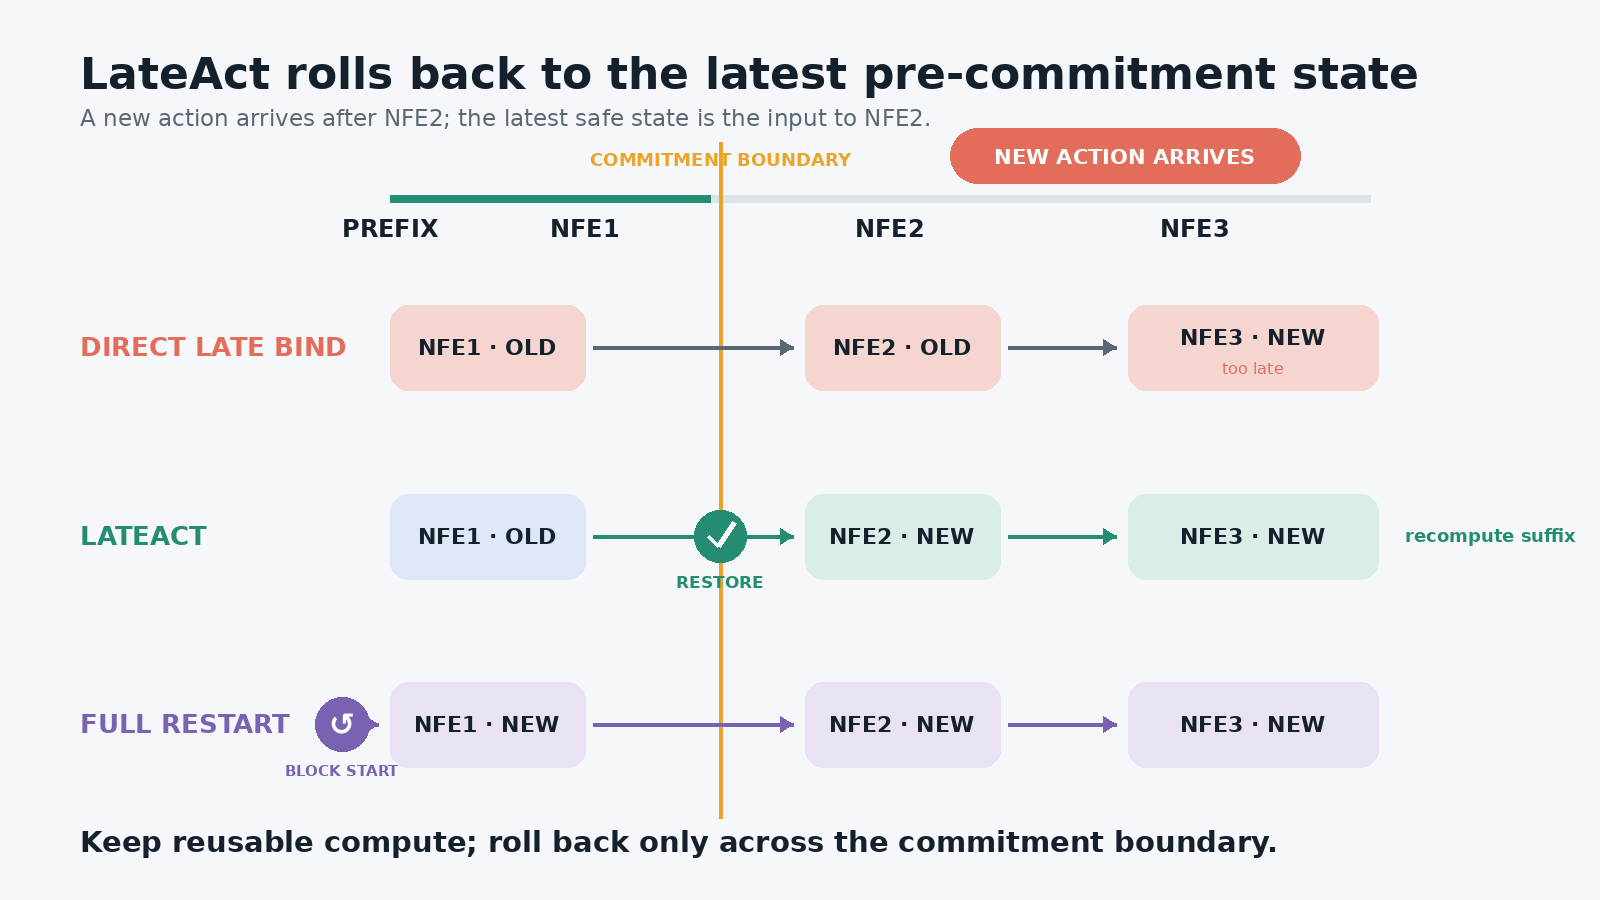
\includegraphics[width=0.84\linewidth]{figures/lateact_mechanism.png}
  \caption{\textbf{\method{} restores the latest pre-commitment state.}
  With a new action arriving after \nfe{}2, direct binding changes only
  \nfe{}3 and remains committed to \old{}. Full restart recomputes all three
  evaluations. \method{} restores the input to \nfe{}2 and recomputes
  \nfe{}2--\nfe{}3 under \new{}, preserving reusable \nfe{}1 work.}
  \label{fig:mechanism}
\end{figure}

\paragraph{Policies.}
Figure~\ref{fig:mechanism} contrasts four serving policies.
\textsc{Next-Block} finishes the current block under \old{} and applies
\new{} only to the next block. \direct{} uses \new{} at the next available
evaluation without restoring state. \restart{} discards current progress and
recomputes all $K$ evaluations under \new{}. \method{} directly binds arrivals
that occur before commitment; otherwise it restores the latest safe state and
replays only the necessary suffix.

\paragraph{Compact exact checkpoint.}
In Matrix-Game, the latest safe point is the input to \nfe{}2. Static and
runtime tracing show that \nfe{}2 overwrites every current-block visual and
action KV position before reading it. Historical-prefix and cross-attention KV
remain immutable. The implemented checkpoint therefore stores the BF16
entering-\nfe{}2 latent ($337{,}920$ bytes) and defensive visual/mouse/keyboard
cache indices ($1{,}440$ bytes), totaling $339{,}360$ bytes. Scheduler state is
stateless for the fixed tensors, and random noise is materialized before
branching. Independent replay audits require bit-exact equality between
restored and freshly generated \old{}-\nfe{}1/\new{}-\nfe{}2--\nfe{}3
trajectories.

\paragraph{Arrival scheduling.}
An action becomes usable after the currently executing evaluation completes.
An arrival during \nfe{}1 binds \new{} for \nfe{}2--\nfe{}3 without restore.
An arrival during \nfe{}2 or \nfe{}3 restores the entering-\nfe{}2 checkpoint
and replays \nfe{}2--\nfe{}3. This fixed rule is calibrated once on disjoint
commitment scenes; the asynchronous evaluation never refits the boundary.

\medskip
\noindent\fbox{\begin{minipage}{0.955\linewidth}
\small
\textbf{Algorithm 1: calibrate and serve with \method{}.}
\textbf{Calibrate:} generate $y_s$ for $s=0{:}K$ with coupled state/noise;
compute $R(s)$ and retain the state at the latest switch $s^*$ passing the
frozen gates. \textbf{Serve:} bind $a_n$ directly if actionable by $s^*$;
otherwise restore $s^*$ and replay only $s^*{+}1{:}K$ under $a_n$.
\textbf{Audit:} trace mutable dependencies read by the suffix to derive the
payload, then verify exact replay.
\end{minipage}}
\medskip

The policy above is architecture-independent; the dependency audit is not.
In particular, neither Matrix-Game's payload nor its 339,360-byte size is
assumed to transfer to another model.

\section{Experimental design}
\label{sec:setup}

\paragraph{Substrates and actions.}
The primary substrate is the open Matrix-Game 2.0 causal generator
\citep{he2025matrixgame2}, evaluated in BF16 with three denoising evaluations
per block. The primary action is opposite mouse-yaw; keyboard A/D is a
pre-specified limitation study. Mechanism replication uses the pinned minWM
Wan2.1 Action2V four-step DMD checkpoint \citep{zhao2026minwm}.

\paragraph{Splits.}
Matrix-Game commitment calibration uses eight official images and both yaw
directions (16 pairs). Minimal rollback uses the same frozen pairs only after
the boundary gate passes. The final serving test uses 32 fresh stochastic
contexts: eight disjoint base images, four deterministic variants per base,
two directions per variant, and 16 deterministic stratified arrivals per
direction (64 direction cells and 1,024 paired arrivals). Statistical
inference clusters by the eight independent base images; the 64 direction
cells remain descriptive quality units.
Keyboard calibration uses 10 fresh stochastic contexts (20 directions), and
its serving confirmation uses 24 disjoint contexts (48 directions).

The original minWM study fixes official prompts 0--7, seeds 41000--41007, and
native lateral \texttt{a*3} versus \texttt{d*3}. Its formal gate fails and is
preserved. After that identifiability audit, exactly one follow-up was frozen
at commit \texttt{f1e2bbc} before its outputs were generated. It uses the same
model, evaluator, thresholds, and gate with stronger native yaw
\texttt{j*3} versus \texttt{l*3}, fresh consecutive official prompts 8--15,
seeds 41008--41015, both directions, and all switch positions
$s=0,\ldots,4$. No scene is screened or replaced, and rollback is prohibited.

\paragraph{Coupling and metrics.}
Every branch shares prefix, initial latent, explicit re-noising tensors,
sampler, weights, historical state, and non-action conditioning; only the
action tensor at designated evaluations differs. Same-action controls must
produce exact latent hashes. Signed horizontal motion is measured with
forward/backward-consistent Lucas--Kanade tracks \citep{lucas1981iterative}
and a RANSAC partial-affine fit \citep{fischler1981ransac}; the second estimate
serves as a complementary sign-consistency check. Keyboard uses the same construction but
an action-appropriate lateral scene-translation score rather than the
mouse-yaw score. Quality uses future-frame SSIM \citep{wang2004ssim}, temporal
consistency, boundary jump, and finite/nonconstant decode checks.
Action-to-pixel latency includes checkpoint operations and VAE decoding.

\paragraph{Frozen gates.}
Matrix-Game requires all 16 directions to be evaluator-valid and a steep,
bounded, monotone response transition. minWM requires an oracle gap of at least
8 pixels, at least $10\times$ the same-action floor, at least 20 median
inliers, and affine/LK sign agreement. Confirmation requires at least 12/16
valid monotone bounded pairs, six per direction, and an adjacent median drop
of 0.15. The thresholds serve distinct safeguards: the 8-pixel gap enforces
absolute action distinguishability, the $10\times$ same-action floor bounds
repeatability noise, the 20-inlier requirement supports estimator stability,
and the 0.15 adjacent-drop gate requires a materially steep transition.
Separately, the 0.10 response tolerance defines operational near-restart
equivalence, while median SSIM $\geq0.90$ serves as the frozen
trajectory-fidelity safeguard. Appendix~\ref{app:quality} gives the full
rationale. All precede broad inference.
Experiments run on two RTX 3090 GPUs for Matrix-Game and one RTX 3090 for
minWM; no training or weight modification is performed.

\section{Results}
\label{sec:results}

\subsection{Denoising-time commitment}

\begin{figure}[t]
  \centering
  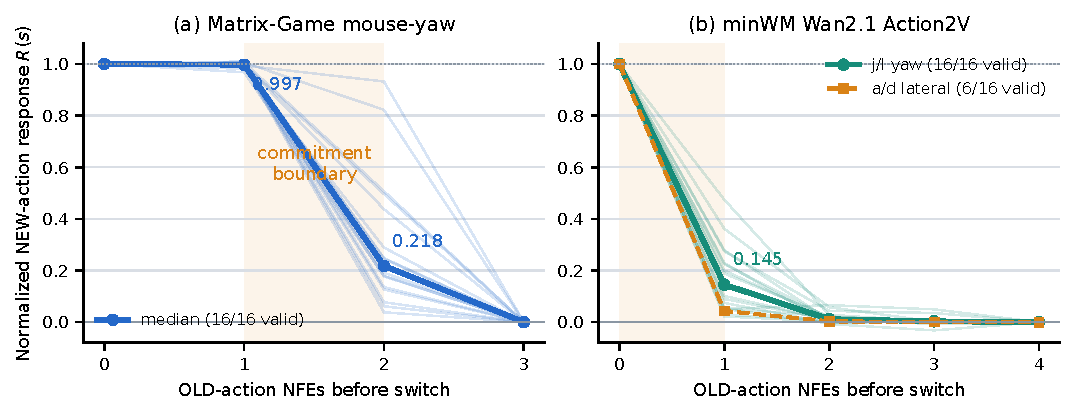
\includegraphics[width=0.92\linewidth]{figures/cross_model_commitment.pdf}
  \caption{\textbf{Action response shows a steep commitment transition at
  few-step sampling granularity.}
  Thin lines are direction-scene curves; bold lines are medians.
  (a) Matrix-Game mouse-yaw retains \new{} after one old-action evaluation
  ($0.997$) but falls to $0.218$ after two (16/16 valid).
  (b) The frozen minWM yaw follow-up passes 16/16 pairs and drops to $0.145$
  after one of four old-action evaluations. The original minWM lateral curve
  is descriptively similar but remains a failed replication because only 6/16
  pairs meet the unchanged oracle-separation gate.}
  \label{fig:curves}
\end{figure}

\paragraph{Matrix-Game.}
All 16 mouse-yaw pairs are valid, monotone, and bounded. Median $R(s)$ for
$s=0,1,2,3$ is $[1.000,0.997,0.218,0.000]$, with a paired median drop of
0.774 from one to two old-action evaluations. This descriptive 16/16 result
places the latest safe checkpoint at the input to \nfe{}2.

\paragraph{Independent minWM mechanism chronology.}
The original eight-scene lateral \texttt{a/d} study passes oracle separation
on only 6/16 pairs (three per direction), below the frozen 12/16 requirement.
Its commitment-like curve is descriptive only; action separation, not the
implementation audits, causes the identifiability failure.

Following this failed identifiability audit, the single pre-specified frozen
\texttt{j/l} yaw follow-up uses fresh prompts and unchanged evaluation,
thresholds, and success gate. It passes 16/16 pairs (8/8 per direction);
all validity and coupling audits pass, and median $R(s)$ is
$[1.000,0.145,0.011,0.003,0.000]$. This replicates the \emph{commitment
mechanism} on a second model, not \method{} rollback or latency; full protocol
and failure chronology appear in Appendix~\ref{app:minwm}.

\subsection{Rollback recovers the new action}

On the 16 Matrix-Game calibration directions, direct binding from the
post-\nfe{}2 state has median response 0.218, while restoring the input to
\nfe{}2 yields 0.997; full restart is 1.000. Minimal rollback improves all
16/16 pairs and is within 0.10 of restart on all 16. Its median future-SSIM to
the new oracle is 0.9026, passing the frozen median-level 0.90 safeguard. A
representative coupled branch is retained in Appendix~\ref{app:quality} rather
than used as primary evidence.

\subsection{Frozen asynchronous serving evaluation}

\begin{table}[t]
  \centering
  \caption{\textbf{Matrix-Game mouse-yaw serving results over 1,024 paired
  arrivals.} Response and latency are descriptive medians. For
  \textsc{Next-Block}, response is for the current block, while latency ends
  when \new{} first affects pixels in the following block. \method{} reaches
  near-restart normalized response with two post-arrival evaluations rather
  than three.}
  \label{tab:serving}
  \small
  \begin{tabular}{lrrrr}
    \toprule
    Policy & Response & Latency (s) & Post-arrival NFEs & Redone NFEs \\
    \midrule
    \textsc{Next-Block} & 0.0000 & 5.1554 & 4 & 0 \\
    \direct{}            & 0.1605 & 2.2925 & 2 & 0 \\
    \restart{}           & 1.0000 & 2.5900 & 3 & 2 \\
    \textbf{\method{}}   & \textbf{0.9999} & \textbf{2.2843} & \textbf{2} & \textbf{1} \\
    \bottomrule
  \end{tabular}
\end{table}

Table~\ref{tab:serving} reports the disjoint serving test. For all 676 arrivals
during \nfe{}2 or \nfe{}3, \method{} is within 0.10 of full restart, redoes
one fewer evaluation, and saves 11.93\% mean late-arrival latency. For all 348
\nfe{}1 arrivals, direct binding and \method{} are the same trajectory, with
zero restore, discard, or redone evaluations.

Inference uses the eight independent base images, not the 64 derived
variant/direction cells. Averaging the actual 676 late-arrival rows within this
hierarchy, \method{} minus \direct{} response is 0.9091 mean and 0.9304 median
across bases (cluster-bootstrap 95\% CI $[0.8598,0.9541]$); all 8/8 base-image
effects are positive. Full-restart minus \method{} latency saving is
0.3118\,s mean and 0.3137\,s median (95\% CI $[0.3055,0.3175]$), again positive
for 8/8 bases. The corresponding exact one-sided Wilcoxon value is
$p=0.0039$ for each effect.

Mouse-yaw trajectory quality is broadly stable but not uniform. Over the 64
descriptive scene-variant/direction comparisons, future-SSIM has median 0.9223
and p05 0.8397; 60/64 are at least 0.85. The frozen $\geq0.90$ requirement is
a median-level safeguard, not a per-direction threshold. Temporal and
finite/nonconstant decode safeguards pass 64/64; Appendix~\ref{app:quality}
discloses the full tail, including the unfavorable 0.7184 minimum.

\paragraph{State and runtime.}
The compact exact checkpoint is 339,360 bytes ($1{,}913\times$ smaller; 1,432
bytes above the logical minimum), with 1.456/0.878\,ms save/restore. All 80
replays pass exact state/scheduler/RNG audits (peak 8.908\,GiB).

\subsection{Keyboard: shared boundary, failed fidelity}

Frozen action-appropriate calibration corrects the initial mouse-yaw score and
finds the \emph{same} boundary: $R(1)=0.9957$, $R(2)=0.1240$. Across 24
contexts, rollback reaches median response 1.0188 and is near restart for all
512 late arrivals, but future-SSIM is 0.6726, below the frozen 0.90 median gate
(temporal 48/48). Shared commitment and direction do not imply action-general
fidelity.

\section{Discussion and limitations}
\label{sec:discussion}

Matrix-Game mouse-yaw supports compact exact rollback with near-restart
response and lower latency. minWM supports mechanism replication only;
\texttt{a/d} remains failed and keyboard precludes action-general fidelity.

\paragraph{Deployment scope.}
Full efficacy is limited to Matrix-Game mouse-yaw; minWM tests commitment, not
rollback/latency. Arrivals are stratified, not production-sampled; latency is
about 2.28\,s; and the boundary is calibrated, not predicted online. No
task-level physical-control objective or real robot is evaluated.

\section{Conclusion}

\method{} turns a measured action-recoverability boundary into exact suffix
replay, yielding near-restart mouse-yaw response with safeguards and lower
Matrix-Game latency. minWM mechanism replication and the negative results
delimit this claim.

\clearpage
\bibliographystyle{plainnat}
\bibliography{references}

\appendix
\section{Frozen protocols and additional results}
\label{app:protocols}

\subsection{Matrix-Game commitment and rollback gates}

\paragraph{Commitment calibration.}
The calibration set contains official universal images 0000--0007 and both
mouse-left$\leftrightarrow$mouse-right directions. For each of the 16
direction-scene pairs, the runner generates the \new{} and \old{} oracles and
the two interior switch points. Prefix, prompt-free image conditioning, initial
current-block latent, future noise tensors, weights, sampler, precision, cache
history, and non-action conditioning are exact across branches. The intended
action tensor is the only difference. All 16 pairs pass oracle distinction,
tracking support, monotonicity, boundedness, temporal quality, and latent
coupling.

\begin{table}[h]
  \centering
  \caption{Frozen Matrix-Game commitment curve. Values are medians over 16
  valid direction-scene pairs.}
  \small
  \begin{tabular}{lrrrr}
    \toprule
    OLD-action NFEs $s$ & 0 & 1 & 2 & 3 \\
    \midrule
    Normalized response $R(s)$ & 1.0000 & 0.9971 & 0.2182 & 0.0000 \\
    \bottomrule
  \end{tabular}
\end{table}

\paragraph{Gate 1 rollback.}
The 16 calibration pairs compare \direct{}, exact rollback of the minimal
suffix, and full restart with identical stochastic inputs. Minimal rollback is within 0.10 of
restart on 16/16 pairs and improves over direct binding on 16/16. Median
responses are 0.2182/0.9971/1.0000 for direct/minimal/restart, and minimal
rollback has median future-SSIM 0.9026.

\subsection{Exact Matrix-Game runtime state}

Matrix-Game routes causal self-attention KV insertion through a single cache
operation immediately before attention reads. Runtime tracing shows that every
current-block visual and active action KV position is overwritten before use
at \nfe{}2. Historical prefix KV and cross-attention KV therefore remain live
by reference rather than being copied.

\begin{table}[h]
  \centering
  \caption{Exact checkpoint storage. The final implementation removes
  overwritten state, not numerical information required by replay.}
  \small
  \begin{tabular}{lr}
    \toprule
    Payload & Bytes \\
    \midrule
    Entering-\nfe{}2 BF16 latent $[1,16,3,44,80]$ & 337,920 \\
    Defensive visual/mouse/keyboard cache indices & 1,440 \\
    \textbf{Implemented exact checkpoint} & \textbf{339,360} \\
    Mathematical minimum (latent plus step) & 337,928 \\
    Initial exact implementation & 649,330,080 \\
    \bottomrule
  \end{tabular}
\end{table}

The final checkpoint is $1{,}913\times$ smaller than the initial
implementation and 1,432 bytes (0.424\%) above the measured logical minimum.
Median save/restore times are 1.456/0.878\,ms. The full live per-fork cache
allocation is 1,670,124,960 bytes but is not duplicated by \method{}.

\subsection{Asynchronous serving details}

The primary serving set uses official images 0008--0015 with four deterministic
prefix-noise variants each. All 32 contexts and both yaw directions are
retained. Each direction receives 16 deterministic stratified-uniform arrival
times over the wall-clock support of the three old-action evaluations, using
one frozen seed family. The resulting classes contain 348 \nfe{}1 arrivals,
338 \nfe{}2 arrivals, and 338 \nfe{}3 arrivals.

The serving hierarchy has eight independent base images, four deterministic
variants per base, two directions per variant, and 16 arrivals per direction.
Late arrivals have \texttt{inflight\_nfe $\geq$ 2}, retaining 676 of 1,024
rows. Inference averages late rows within direction and the eight derived
variant/direction cells within each base, then treats the eight base images as
clusters. The late-arrival \method{}-minus-\direct{} response effect has mean
0.909136, median 0.930385, and base-cluster bootstrap 95\% CI
$[0.859769,0.954093]$; all 8/8 base effects are positive (exact one-/two-sided
Wilcoxon $p=0.00390625/0.0078125$). The fixed per-direction
\texttt{lateact-direct\_late} branch contrast is a distinct descriptive
$n=64$ estimand (mean 0.815919), not the mean over the 676 asynchronous late
rows.

Full-restart-minus-\method{} latency saving across the eight base clusters has
mean 0.311789\,s, median 0.313654\,s, and 95\% CI
$[0.305519,0.317523]$\,s; 8/8 are positive with the same exact Wilcoxon
values. The frozen mean saving fraction is 11.93\%. Every late case is within
0.10 normalized response of restart and uses fewer redone evaluations. All
348 early cases use exactly zero rollback.

\subsection{Mouse-yaw trajectory-quality tail}
\label{app:quality}

The 64 scene-variant/direction comparisons are descriptive quality units. The
future-SSIM distribution has mean 0.915660, median 0.922305, p05 0.839679, and
minimum 0.718375. Counts at least 0.90/0.85/0.80 are 49/64, 60/64, and 63/64;
equivalently 15/64, 4/64, and 1/64 fall below those values. Sub-0.90 values
occur in four base images; base 0013 contains 6/8 and the sole value below
0.80. Thus mouse-yaw trajectory quality is broadly stable but not uniform.
The frozen SSIM $\geq0.90$ gate is a median-level safeguard, not a per-example
threshold, and no tail cutoff is introduced retrospectively.

Temporal difference (\method{} minus \new{}) has median +0.001691 and range
$[-0.007878,0.018057]$; temporal and finite/nonconstant decode safeguards pass
64/64.

\begin{figure}[h]
  \centering
  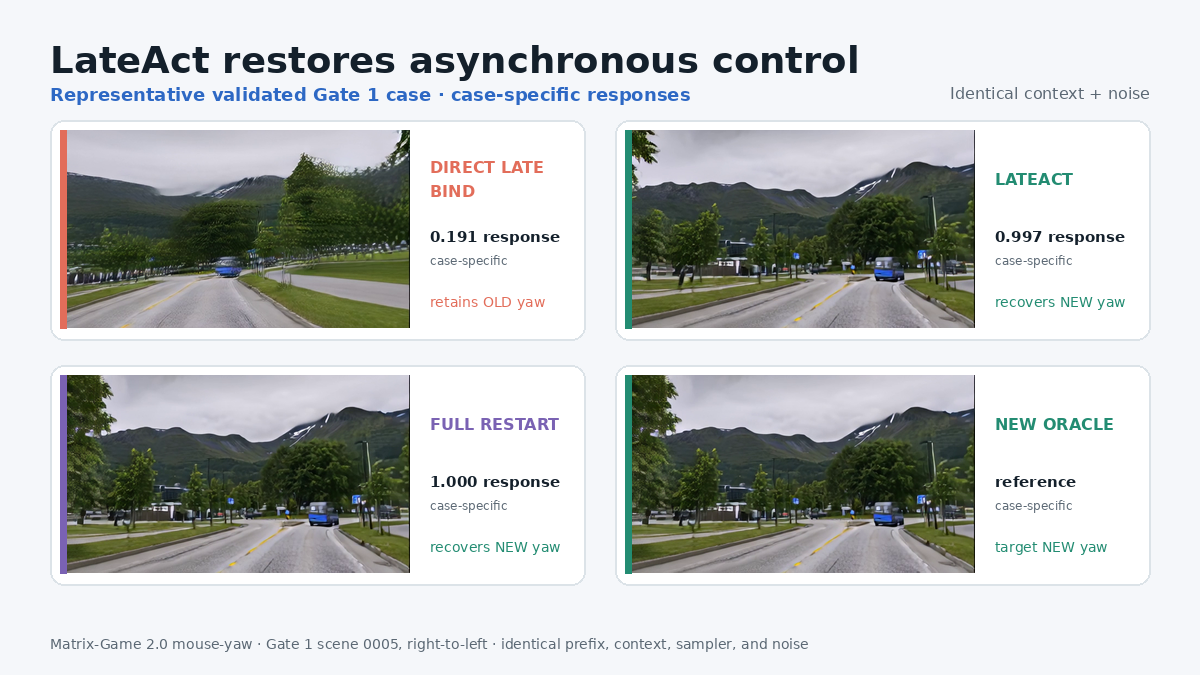
\includegraphics[width=0.72\linewidth]{figures/matrix_qualitative.png}
  \caption{Representative coupled Matrix-Game mouse-yaw branch. Direct late
  binding retains the old yaw (response 0.191), while \method{} (0.997) tracks
  full restart (1.000) in normalized action response. This favorable example
  is not the quality-tail evidence and was not used to set thresholds.}
  \label{fig:qualitative}
\end{figure}

\subsection{Gate rationale}

The frozen numerical cutoffs are safeguards against specific invalidating
conditions, not uniquely privileged constants. The 8-pixel oracle gap demands
minimum absolute action separation; the $10\times$ same-action floor demands
separation well above repeatability noise; and at least 20 motion inliers
protects the affine estimate from sparse tracking. A 0.10 normalized-response
gap is the operational near-restart tolerance. Median future-SSIM $\geq0.90$
protects trajectory fidelity without requiring every example to exceed 0.90.
Finally, a median adjacent response drop of at least 0.15 distinguishes a
materially steep transition at the available NFE granularity from a flat or
noisy curve.

\subsection{minWM frozen chronology}
\label{app:minwm}

\paragraph{Original lateral control.}
The original minWM protocol fixes prompts 0--7, seeds 41000--41007, actions
\texttt{a*3}/\texttt{d*3}, both directions, and $s=0,\ldots,4$. The
same-action decoded floor is 0.0776 pixels. Oracle affine gaps have median
6.851 pixels and range 1.169--12.767; only three scenes in both directions
exceed the fixed 8-pixel threshold, yielding 6/16 valid pairs. The
formal replication verdict is failure even though all 16 raw curves are
monotone and bounded and show a median first drop of 0.9566.

\paragraph{Frozen yaw confirmation.}
After the lateral identifiability failure was established, exactly one bounded
follow-up protocol was frozen at commit \texttt{f1e2bbc} before confirmatory
outputs were generated. It fixes fresh consecutive official prompts 8--15,
seeds 41008--41015, native \texttt{j*3}/\texttt{l*3} yaw, both switch
directions, the unchanged evaluator, thresholds, and success gate. Prompt
screening/replacement, alternative evaluators or actions, and rollback are
prohibited. This is a pre-specified frozen follow-up after a failed
identifiability audit; the adaptive chronology is explicit, and the protocol
was fixed before confirmatory execution.

\begin{table}[h]
  \centering
  \caption{Per-scene minWM yaw oracle separation. The signed value reverses
  between directions; absolute gap and inlier support are shared.}
  \small
  \begin{tabular}{lrrc}
    \toprule
    Scene & Absolute gap (px) & Median oracle inliers & Valid directions \\
    \midrule
    08 & 35.359 & 177.0 & 2/2 \\
    09 & 14.002 & 833.5 & 2/2 \\
    10 & 13.982 & 690.5 & 2/2 \\
    11 & 35.345 & 469.5 & 2/2 \\
    12 & 10.238 & 298.5 & 2/2 \\
    13 & 19.007 & 246.0 & 2/2 \\
    14 & 19.035 & 631.5 & 2/2 \\
    15 & 45.441 & 399.5 & 2/2 \\
    \bottomrule
  \end{tabular}
\end{table}

The same-action control ranges are 0.3892 and 0.6580 pixels; the latter is the
frozen repeatability floor, giving a $10\times$ requirement of 6.5801 pixels.
All 16 pairs exceed both this value and 8 pixels. Affine/LK signs agree 16/16,
all median inlier counts exceed 20, all videos are valid, and all 16 curves are
monotone and bounded. Exact branch-noise hashes, historical/cross-sampled
state, and four-evaluation counts pass on all eight scenes. Same-action latent
hashes are exact on both control prompts.

\subsection{Keyboard chronology}
\label{app:keyboard}

The initial eight-context keyboard transfer used the mouse-yaw score and
reported asymmetric response. The subsequent diagnostic froze an
action-appropriate signed lateral translation evaluator before generating
broad results. On 10 calibration contexts and 20 directions, all directions
are valid; median response is 0.9957 at $s=1$ and 0.1240 at $s=2$, placing the
latest safe state after \nfe{}1, exactly as for mouse-yaw.

The confirmation uses 24 disjoint stochastic contexts, 48 directions, and 16
arrivals per direction. Mouse-boundary and action-specific policies are the
same algorithm and are bit-exact on 768/768 records. Median response is 1.0188;
all 512 late arrivals are within 0.10 of restart and save 0.3105\,s median.
Nevertheless, median future-SSIM to \new{} is 0.6726 (range
0.5989--0.9139), failing the frozen median-level 0.90 threshold. Temporal consistency passes
48/48. The videos are coherent but follow a different exact trajectory.

\section{Reproducibility and audit details}
\label{app:repro}
\label{app:audits}
\label{app:compute}

No model is trained or fine-tuned. The experiments use released Matrix-Game
2.0 and minWM Wan2.1 Action2V checkpoints, BF16 inference, deterministic
materialized future noise, and frozen YAML protocols. Runners, analyzers,
protocol validators, configs, and lightweight reports are retained for an
anonymous release; large checkpoints and generated videos are excluded.

For each scientific branch, the runner records hashes of action tensors,
initial and re-noising tensors, prefix latents, cache indices, sampled
historical cache bytes, cross-attention state, and output latents. Analyzer
guards reject prompt substitution, action mismatch, threshold drift, output
overwrite, insufficient oracle separation, evaluator-sign disagreement,
non-finite videos, and failed same-action equality.

Matrix-Game generation uses two NVIDIA RTX 3090 GPUs. The primary serving
runner measures 955.60 synchronized GPU-seconds across 64 scene-directions
(6.21\,s generation and 8.72\,s decode per bundle). minWM uses one RTX 3090;
74 confirmatory branches average 6.156\,s generation and 7.417\,s decode
(1,004.42 timed GPU-seconds total), with 19,340,754,432 peak allocated bytes.

\section{Existing assets and broader impact}
\label{app:impact}

The work evaluates released Matrix-Game 2.0 and minWM implementations and
checkpoints and cites their corresponding papers. The Matrix-Game 2.0 source
release identifies an MIT license; minWM is released under Apache-2.0. Model
checkpoints and official evaluation assets are used under their respective
upstream terms and are not redistributed in the submission.

Commitment-aware rollback can reduce wasted inference and make interactive
world-model feedback more responsive, which may benefit embodied-agent
simulation and human-in-the-loop control. The same capability can also make
synthetic environments more persuasive despite incorrect dynamics. A
particularly relevant failure mode is false confidence: recovering an
action-direction metric does not guarantee recovery of the exact intended
trajectory, as demonstrated by the keyboard SSIM failure. These systems should
therefore not control safety-critical physical hardware solely from the
evaluated pixel or motion metrics. Deployment would require task-level state
validation, uncertainty monitoring, safe fallback behavior, and evaluation on
the target embodiment.


\section*{NeurIPS Paper Checklist}


\begin{enumerate}

\item {\bf Claims}
    \item[] Question: Do the main claims made in the abstract and introduction accurately reflect the paper's contributions and scope?
    \item[] Answer: \answerYes{}
    \item[] Justification: The abstract and Sections~\ref{sec:intro} and~\ref{sec:results} distinguish Matrix-Game rollback efficacy from the narrower minWM mechanism replication; Section~\ref{sec:discussion} states the non-universal scope explicitly.
    \item[] Guidelines:
    \begin{itemize}
        \item The answer \answerNA{} means that the abstract and introduction do not include the claims made in the paper.
        \item The abstract and/or introduction should clearly state the claims made, including the contributions made in the paper and important assumptions and limitations. A \answerNo{} or \answerNA{} answer to this question will not be perceived well by the reviewers. 
        \item The claims made should match theoretical and experimental results, and reflect how much the results can be expected to generalize to other settings. 
        \item It is fine to include aspirational goals as motivation as long as it is clear that these goals are not attained by the paper. 
    \end{itemize}

\item {\bf Limitations}
    \item[] Question: Does the paper discuss the limitations of the work performed by the authors?
    \item[] Answer: \answerYes{}
    \item[] Justification: Section~\ref{sec:discussion} and Appendix~\ref{app:keyboard} discuss the model-, action-, and evaluator-specific limitations, including the failed keyboard trajectory-fidelity gate.
    \item[] Guidelines:
    \begin{itemize}
        \item The answer \answerNA{} means that the paper has no limitation while the answer \answerNo{} means that the paper has limitations, but those are not discussed in the paper. 
        \item The authors are encouraged to create a separate ``Limitations'' section in their paper.
        \item The paper should point out any strong assumptions and how robust the results are to violations of these assumptions (e.g., independence assumptions, noiseless settings, model well-specification, asymptotic approximations only holding locally). The authors should reflect on how these assumptions might be violated in practice and what the implications would be.
        \item The authors should reflect on the scope of the claims made, e.g., if the approach was only tested on a few datasets or with a few runs. In general, empirical results often depend on implicit assumptions, which should be articulated.
        \item The authors should reflect on the factors that influence the performance of the approach. For example, a facial recognition algorithm may perform poorly when image resolution is low or images are taken in low lighting. Or a speech-to-text system might not be used reliably to provide closed captions for online lectures because it fails to handle technical jargon.
        \item The authors should discuss the computational efficiency of the proposed algorithms and how they scale with dataset size.
        \item If applicable, the authors should discuss possible limitations of their approach to address problems of privacy and fairness.
        \item While the authors might fear that complete honesty about limitations might be used by reviewers as grounds for rejection, a worse outcome might be that reviewers discover limitations that aren't acknowledged in the paper. The authors should use their best judgment and recognize that individual actions in favor of transparency play an important role in developing norms that preserve the integrity of the community. Reviewers will be specifically instructed to not penalize honesty concerning limitations.
    \end{itemize}

\item {\bf Theory assumptions and proofs}
    \item[] Question: For each theoretical result, does the paper provide the full set of assumptions and a complete (and correct) proof?
    \item[] Answer: \answerNA{}
    \item[] Justification: The paper makes no formal theoretical claim and presents no theorem or proof.
    \item[] Guidelines:
    \begin{itemize}
        \item The answer \answerNA{} means that the paper does not include theoretical results. 
        \item All the theorems, formulas, and proofs in the paper should be numbered and cross-referenced.
        \item All assumptions should be clearly stated or referenced in the statement of any theorems.
        \item The proofs can either appear in the main paper or the supplemental material, but if they appear in the supplemental material, the authors are encouraged to provide a short proof sketch to provide intuition. 
        \item Inversely, any informal proof provided in the core of the paper should be complemented by formal proofs provided in appendix or supplemental material.
        \item Theorems and Lemmas that the proof relies upon should be properly referenced. 
    \end{itemize}

    \item {\bf Experimental result reproducibility}
    \item[] Question: Does the paper fully disclose all the information needed to reproduce the main experimental results of the paper to the extent that it affects the main claims and/or conclusions of the paper (regardless of whether the code and data are provided or not)?
    \item[] Answer: \answerYes{}
    \item[] Justification: Sections~\ref{sec:problem}--\ref{sec:setup} and Appendix~\ref{app:protocols}--\ref{app:audits} specify the interventions, fixed thresholds, seeds, prompts, timing protocol, metrics, and frozen failure chronology needed to reproduce the claims.
    \item[] Guidelines:
    \begin{itemize}
        \item The answer \answerNA{} means that the paper does not include experiments.
        \item If the paper includes experiments, a \answerNo{} answer to this question will not be perceived well by the reviewers: Making the paper reproducible is important, regardless of whether the code and data are provided or not.
        \item If the contribution is a dataset and\slash or model, the authors should describe the steps taken to make their results reproducible or verifiable. 
        \item Depending on the contribution, reproducibility can be accomplished in various ways. For example, if the contribution is a novel architecture, describing the architecture fully might suffice, or if the contribution is a specific model and empirical evaluation, it may be necessary to either make it possible for others to replicate the model with the same dataset, or provide access to the model. In general. releasing code and data is often one good way to accomplish this, but reproducibility can also be provided via detailed instructions for how to replicate the results, access to a hosted model (e.g., in the case of a large language model), releasing of a model checkpoint, or other means that are appropriate to the research performed.
        \item While NeurIPS does not require releasing code, the conference does require all submissions to provide some reasonable avenue for reproducibility, which may depend on the nature of the contribution. For example
        \begin{enumerate}
            \item If the contribution is primarily a new algorithm, the paper should make it clear how to reproduce that algorithm.
            \item If the contribution is primarily a new model architecture, the paper should describe the architecture clearly and fully.
            \item If the contribution is a new model (e.g., a large language model), then there should either be a way to access this model for reproducing the results or a way to reproduce the model (e.g., with an open-source dataset or instructions for how to construct the dataset).
            \item We recognize that reproducibility may be tricky in some cases, in which case authors are welcome to describe the particular way they provide for reproducibility. In the case of closed-source models, it may be that access to the model is limited in some way (e.g., to registered users), but it should be possible for other researchers to have some path to reproducing or verifying the results.
        \end{enumerate}
    \end{itemize}


\item {\bf Open access to data and code}
    \item[] Question: Does the paper provide open access to the data and code, with sufficient instructions to faithfully reproduce the main experimental results, as described in supplemental material?
    \item[] Answer: \answerNo{}
    \item[] Justification: An anonymous, self-contained code archive is not included with this submission; the implementation depends on separately licensed upstream models. The paper supplies detailed protocols and frozen configurations.
    \item[] Guidelines:
    \begin{itemize}
        \item The answer \answerNA{} means that paper does not include experiments requiring code.
        \item Please see the NeurIPS code and data submission guidelines (\url{https://neurips.cc/public/guides/CodeSubmissionPolicy}) for more details.
        \item While we encourage the release of code and data, we understand that this might not be possible, so \answerNo{} is an acceptable answer. Papers cannot be rejected simply for not including code, unless this is central to the contribution (e.g., for a new open-source benchmark).
        \item The instructions should contain the exact command and environment needed to run to reproduce the results. See the NeurIPS code and data submission guidelines (\url{https://neurips.cc/public/guides/CodeSubmissionPolicy}) for more details.
        \item The authors should provide instructions on data access and preparation, including how to access the raw data, preprocessed data, intermediate data, and generated data, etc.
        \item The authors should provide scripts to reproduce all experimental results for the new proposed method and baselines. If only a subset of experiments are reproducible, they should state which ones are omitted from the script and why.
        \item At submission time, to preserve anonymity, the authors should release anonymized versions (if applicable).
        \item Providing as much information as possible in supplemental material (appended to the paper) is recommended, but including URLs to data and code is permitted.
    \end{itemize}


\item {\bf Experimental setting/details}
    \item[] Question: Does the paper specify all the training and test details (e.g., data splits, hyperparameters, how they were chosen, type of optimizer) necessary to understand the results?
    \item[] Answer: \answerYes{}
    \item[] Justification: Section~\ref{sec:setup} and Appendix~\ref{app:protocols}--\ref{app:minwm} provide the model variants, actions, context sets, seeds, switch positions, metrics, and all frozen decision thresholds.
    \item[] Guidelines:
    \begin{itemize}
        \item The answer \answerNA{} means that the paper does not include experiments.
        \item The experimental setting should be presented in the core of the paper to a level of detail that is necessary to appreciate the results and make sense of them.
        \item The full details can be provided either with the code, in appendix, or as supplemental material.
    \end{itemize}

\item {\bf Experiment statistical significance}
    \item[] Question: Does the paper report error bars suitably and correctly defined or other appropriate information about the statistical significance of the experiments?
    \item[] Answer: \answerYes{}
    \item[] Justification: Results are reported over all frozen contexts or direction--scene pairs, with paired medians, complete pass counts, and individual curves rather than selected examples; the exact units of variation are stated in Sections~\ref{sec:setup}--\ref{sec:results}.
    \item[] Guidelines:
    \begin{itemize}
        \item The answer \answerNA{} means that the paper does not include experiments.
        \item The authors should answer \answerYes{} if the results are accompanied by error bars, confidence intervals, or statistical significance tests, at least for the experiments that support the main claims of the paper.
        \item The factors of variability that the error bars are capturing should be clearly stated (for example, train/test split, initialization, random drawing of some parameter, or overall run with given experimental conditions).
        \item The method for calculating the error bars should be explained (closed form formula, call to a library function, bootstrap, etc.)
        \item The assumptions made should be given (e.g., Normally distributed errors).
        \item It should be clear whether the error bar is the standard deviation or the standard error of the mean.
        \item It is OK to report 1-sigma error bars, but one should state it. The authors should preferably report a 2-sigma error bar than state that they have a 96\% CI, if the hypothesis of Normality of errors is not verified.
        \item For asymmetric distributions, the authors should be careful not to show in tables or figures symmetric error bars that would yield results that are out of range (e.g., negative error rates).
        \item If error bars are reported in tables or plots, the authors should explain in the text how they were calculated and reference the corresponding figures or tables in the text.
    \end{itemize}

\item {\bf Experiments compute resources}
    \item[] Question: For each experiment, does the paper provide sufficient information on the computer resources (type of compute workers, memory, time of execution) needed to reproduce the experiments?
    \item[] Answer: \answerYes{}
    \item[] Justification: Appendix~\ref{app:compute} reports GPU type and memory, model precision, measured per-sample generation times, and the scope of both reported and failed experiments.
    \item[] Guidelines:
    \begin{itemize}
        \item The answer \answerNA{} means that the paper does not include experiments.
        \item The paper should indicate the type of compute workers CPU or GPU, internal cluster, or cloud provider, including relevant memory and storage.
        \item The paper should provide the amount of compute required for each of the individual experimental runs as well as estimate the total compute. 
        \item The paper should disclose whether the full research project required more compute than the experiments reported in the paper (e.g., preliminary or failed experiments that didn't make it into the paper). 
    \end{itemize}
    
\item {\bf Code of ethics}
    \item[] Question: Does the research conducted in the paper conform, in every respect, with the NeurIPS Code of Ethics \url{https://neurips.cc/public/EthicsGuidelines}?
    \item[] Answer: \answerYes{}
    \item[] Justification: The research uses released models and synthetic game-like assets, involves no human subjects or private data, and preserves double-blind anonymity.
    \item[] Guidelines:
    \begin{itemize}
        \item The answer \answerNA{} means that the authors have not reviewed the NeurIPS Code of Ethics.
        \item If the authors answer \answerNo, they should explain the special circumstances that require a deviation from the Code of Ethics.
        \item The authors should make sure to preserve anonymity (e.g., if there is a special consideration due to laws or regulations in their jurisdiction).
    \end{itemize}


\item {\bf Broader impacts}
    \item[] Question: Does the paper discuss both potential positive societal impacts and negative societal impacts of the work performed?
    \item[] Answer: \answerYes{}
    \item[] Justification: Appendix~\ref{app:impact} discusses efficiency and responsiveness benefits as well as risks from false confidence in visually plausible but dynamically incorrect predictions, with suggested deployment safeguards.
    \item[] Guidelines:
    \begin{itemize}
        \item The answer \answerNA{} means that there is no societal impact of the work performed.
        \item If the authors answer \answerNA{} or \answerNo, they should explain why their work has no societal impact or why the paper does not address societal impact.
        \item Examples of negative societal impacts include potential malicious or unintended uses (e.g., disinformation, generating fake profiles, surveillance), fairness considerations (e.g., deployment of technologies that could make decisions that unfairly impact specific groups), privacy considerations, and security considerations.
        \item The conference expects that many papers will be foundational research and not tied to particular applications, let alone deployments. However, if there is a direct path to any negative applications, the authors should point it out. For example, it is legitimate to point out that an improvement in the quality of generative models could be used to generate Deepfakes for disinformation. On the other hand, it is not needed to point out that a generic algorithm for optimizing neural networks could enable people to train models that generate Deepfakes faster.
        \item The authors should consider possible harms that could arise when the technology is being used as intended and functioning correctly, harms that could arise when the technology is being used as intended but gives incorrect results, and harms following from (intentional or unintentional) misuse of the technology.
        \item If there are negative societal impacts, the authors could also discuss possible mitigation strategies (e.g., gated release of models, providing defenses in addition to attacks, mechanisms for monitoring misuse, mechanisms to monitor how a system learns from feedback over time, improving the efficiency and accessibility of ML).
    \end{itemize}
    
\item {\bf Safeguards}
    \item[] Question: Does the paper describe safeguards that have been put in place for responsible release of data or models that have a high risk for misuse (e.g., pre-trained language models, image generators, or scraped datasets)?
    \item[] Answer: \answerNA{}
    \item[] Justification: This work releases no new pretrained model, scraped dataset, or other high-risk generative asset; it evaluates existing research checkpoints.
    \item[] Guidelines:
    \begin{itemize}
        \item The answer \answerNA{} means that the paper poses no such risks.
        \item Released models that have a high risk for misuse or dual-use should be released with necessary safeguards to allow for controlled use of the model, for example by requiring that users adhere to usage guidelines or restrictions to access the model or implementing safety filters. 
        \item Datasets that have been scraped from the Internet could pose safety risks. The authors should describe how they avoided releasing unsafe images.
        \item We recognize that providing effective safeguards is challenging, and many papers do not require this, but we encourage authors to take this into account and make a best faith effort.
    \end{itemize}

\item {\bf Licenses for existing assets}
    \item[] Question: Are the creators or original owners of assets (e.g., code, data, models), used in the paper, properly credited and are the license and terms of use explicitly mentioned and properly respected?
    \item[] Answer: \answerYes{}
    \item[] Justification: Appendix~\ref{app:impact} credits Matrix-Game 2.0 and minWM, names their MIT and Apache-2.0 source licenses, and states that upstream checkpoints/assets are not redistributed.
    \item[] Guidelines:
    \begin{itemize}
        \item The answer \answerNA{} means that the paper does not use existing assets.
        \item The authors should cite the original paper that produced the code package or dataset.
        \item The authors should state which version of the asset is used and, if possible, include a URL.
        \item The name of the license (e.g., CC-BY 4.0) should be included for each asset.
        \item For scraped data from a particular source (e.g., website), the copyright and terms of service of that source should be provided.
        \item If assets are released, the license, copyright information, and terms of use in the package should be provided. For popular datasets, \url{paperswithcode.com/datasets} has curated licenses for some datasets. Their licensing guide can help determine the license of a dataset.
        \item For existing datasets that are re-packaged, both the original license and the license of the derived asset (if it has changed) should be provided.
        \item If this information is not available online, the authors are encouraged to reach out to the asset's creators.
    \end{itemize}

\item {\bf New assets}
    \item[] Question: Are new assets introduced in the paper well documented and is the documentation provided alongside the assets?
    \item[] Answer: \answerNA{}
    \item[] Justification: The paper introduces an inference method and evaluation protocols, not a new dataset or pretrained model asset.
    \item[] Guidelines:
    \begin{itemize}
        \item The answer \answerNA{} means that the paper does not release new assets.
        \item Researchers should communicate the details of the dataset\slash code\slash model as part of their submissions via structured templates. This includes details about training, license, limitations, etc. 
        \item The paper should discuss whether and how consent was obtained from people whose asset is used.
        \item At submission time, remember to anonymize your assets (if applicable). You can either create an anonymized URL or include an anonymized zip file.
    \end{itemize}

\item {\bf Crowdsourcing and research with human subjects}
    \item[] Question: For crowdsourcing experiments and research with human subjects, does the paper include the full text of instructions given to participants and screenshots, if applicable, as well as details about compensation (if any)? 
    \item[] Answer: \answerNA{}
    \item[] Justification: The work includes neither crowdsourcing nor human-subject research.
    \item[] Guidelines:
    \begin{itemize}
        \item The answer \answerNA{} means that the paper does not involve crowdsourcing nor research with human subjects.
        \item Including this information in the supplemental material is fine, but if the main contribution of the paper involves human subjects, then as much detail as possible should be included in the main paper. 
        \item According to the NeurIPS Code of Ethics, workers involved in data collection, curation, or other labor should be paid at least the minimum wage in the country of the data collector. 
    \end{itemize}

\item {\bf Institutional review board (IRB) approvals or equivalent for research with human subjects}
    \item[] Question: Does the paper describe potential risks incurred by study participants, whether such risks were disclosed to the subjects, and whether Institutional Review Board (IRB) approvals (or an equivalent approval/review based on the requirements of your country or institution) were obtained?
    \item[] Answer: \answerNA{}
    \item[] Justification: The work includes no human participants and therefore requires no IRB review.
    \item[] Guidelines:
    \begin{itemize}
        \item The answer \answerNA{} means that the paper does not involve crowdsourcing nor research with human subjects.
        \item Depending on the country in which research is conducted, IRB approval (or equivalent) may be required for any human subjects research. If you obtained IRB approval, you should clearly state this in the paper. 
        \item We recognize that the procedures for this may vary significantly between institutions and locations, and we expect authors to adhere to the NeurIPS Code of Ethics and the guidelines for their institution. 
        \item For initial submissions, do not include any information that would break anonymity (if applicable), such as the institution conducting the review.
    \end{itemize}

\item {\bf Declaration of LLM usage}
    \item[] Question: Does the paper describe the usage of LLMs if it is an important, original, or non-standard component of the core methods in this research? Note that if the LLM is used only for writing, editing, or formatting purposes and does \emph{not} impact the core methodology, scientific rigor, or originality of the research, declaration is not required.
    %this research? 
    \item[] Answer: \answerNA{}
    \item[] Justification: LLMs are not an important, original, or non-standard component of the method, experiments, or scientific evidence.
    \item[] Guidelines:
    \begin{itemize}
        \item The answer \answerNA{} means that the core method development in this research does not involve LLMs as any important, original, or non-standard components.
        \item Please refer to our LLM policy in the NeurIPS handbook for what should or should not be described.
    \end{itemize}

\end{enumerate}


\end{document}
